\chapter{Planificación}
\title{Planificación}

\title{Metodología de desarrollo}
\section{Metodología de desarrollo}

\paragraph{
La metodología que se ha tratado de seguir para el desarrollo de este proyecto ha sido
un modelo en espiral ya que lo primero que se quiere solucionar es una funcionalidad
básica (mantener el mismo pulso entre todos los músicos). Sobre esto,
se desea que la comunidad (o los mismos desarrolladores), introduzcan nuevas
funcionalidades.
}

\paragraph{
Incluso dentro del desarrollo de la funcionalidad más básica (que es
la que se trata de implementar en este trabajo), se sigue el una metodología en espiral:
}

\begin{enumerate}
  \item Extracción de los requisitos
  \item Planificación
  \item Ingeniería
  \item Construcción
\end{enumerate}

\title{Fases}
\section{Fases}
\paragraph{
En la anterior sección se ha comentado la metodología a utilizar y, de forma general,
las fases a desarrollar. En esta sección se va a entrar en más detalle.
}

\begin{description}
  \item [Extracción de los requisitos]\hfill \\
  \begin{itemize}
    \item Descripción: obtención de los requisitos funcionales, no funcionales y de información del proyecto
    \item Apartado: Capítulo \ref{cap:EspecificaciondeRequisitos}
  \end{itemize}
  \item [Planificación]\hfill \\
    \begin{itemize}
      \item Descripción: estimación de costo, temporal, recursos humanos...
      \item Apartado: Este capítulo
    \end{itemize}
  \item [Ingeniería]\hfill \\
  \begin{itemize}
    \item Descripción: análisis de los requisitos y diseño del sistema a desarrollar
    \item Apartado: Capítulos \ref{cap:Analisis} y  \ref{cap:Diseno}
  \end{itemize}
  \item [Construcción]\hfill \\
  \item Descripción: implementación del proyecto
  \item Apartado: Capítulo \ref{cap:Implementacion}
\end{description}

\title{Estimación temporal}
\section{Estimación temporal}
\paragraph{
Teniendo en cuenta las partes detalladas en las sección anterior, es momento de
hacer una estimación temporal del proyecto.
}

\begin{itemize}
  \item Especificaciones del proyecto
  \begin{itemize}
    \item{Conocer adecuadamente las necesidades del usuario}
    \item{Establecer los objetivos del proyecto}
    \item{Extraer requisitos funcionales}
    \item{Extraer requisitos no funcionales}
    \item{Extraer requisitos de información}
    \item{Tiempo estimado: \textbf{15 horas}}
  \end{itemize}
\end{itemize}

\begin{itemize}
  \item Planificación
  \begin{itemize}
    \item{Calcular un presupuesto}
    \item{Establecer una temporización}
    \item{Establecer las fases}
    \item{Encontrar recursos que puedan ser reutilizables en el proyecto}
    \item{Definir los recursos humanos disponibles}
    \item{Tiempo estimado: \textbf{20 horas}}
  \end{itemize}
\end{itemize}

\begin{itemize}
  \item Análisis y diseño
  \begin{itemize}
    \item{Analizar los requisitos del proyecto}
    \item{Creación de diagramas}
    \item{Diseño de arquitectura}
    \item{Tiempo estimado: \textbf{40 horas}}
  \end{itemize}
\end{itemize}


\begin{itemize}
  \item Construcción
  \begin{itemize}
    \item{Establecer herramientas/plataformas/lenguaje/software a utilizar}
      \begin{itemize}
        \item{Decidir qué plataformas utilizar}
        \item{Investigar las herramientas de desarrollo de las plataformas}
        \item{Realizar pruebas para conocer si las plataformas son válidas para el proyecto}
      \end{itemize}
    \item{Comunicación entre los actores del sistema}
    \item{Cálculo de los valores necesarios para mantener el tempo en un actor}
    \item{Envío del tempo desde el director a los músicos}
    \item{Posibilidad de cambiar el tempo (por parte del director)}
    \item{Aplicaciones propias para cambiar el tempo}
    \item{Tiempo estimado: \textbf{100 horas}}
  \end{itemize}
\end{itemize}

\begin{itemize}
  \item Documentación
  \begin{itemize}
    \item{Documentar código}
    \item{Documentación del proyecto}
    \item{Creación de esquemas eléctricos para ayudar a futuros desarrolladores
    a comprender el conexionado}
    \item{Tiempo estimado: \textbf{40 horas}}
  \end{itemize}
\end{itemize}

\paragraph{
Se ha hecho una estimación de la cantidad de días que ocuparían todas
estas tareas y, para mostrarlo de una forma más gráfica,
se ha creado un diagrama de Grantt, que se puede ver en la figura \ref{fig:grantt}.
}

\begin{figure}[htb]
\centering
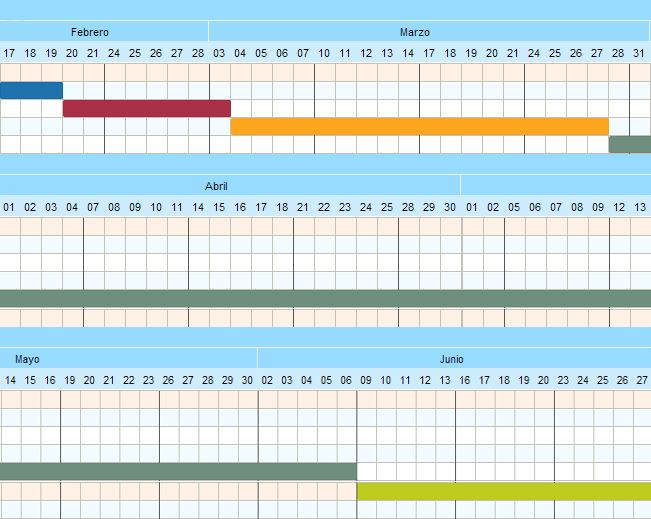
\includegraphics[width=1\textwidth]{./imagenes/grantt}
\caption{Diagrama de Grantt} \label{fig:grantt}
\end{figure}


\title{Recursos humanos}
\section{Recursos humanos}

\paragraph{
Gracias a que es un proyecto de software/hardware libre, todo aquel que
desee particiar en el proyecto puede hacerlo realizando aportaciones en los
\href{https://github.com/iblancasa/ArduBand}{repositorios del proyecto}.
}


\title{Recursos reutilizables}
\section{Recursos técnicos reutilizables}

\paragraph{
Estos recursos hacen referencia a anteriores desarrollos hardware o software creados
por otros desarrolladores o empresas.
}

\paragraph{
En el capítulo de implementación se explicará con más detalle por qué se
eligen los elementos que se van a describir en los dos siguientes apartados.
}


\subsection{Recursos software reutilizables}
\title{Recursos software reutilizable}


\paragraph{
En la introducción se hacía hincapié en la necesidad de crear una aplicación
Android para ayudar al director a establecer el tempo deseado. Por tanto,
serán recursos a tener en cuenta durante el desarrollo todas las herramientas
que implementa el propio SDK de Android y aquellas bibliotecas con licencia
libre que se encuentran en Internet (ya sean para añadir funcionalidad o elementos
gráficos).
}

\paragraph{
También se va a desarrollar un dispositivo físico que necesitará un software para estar
controlado. Todas las bibliotecas del controlador con licencia libre, también estarán
disponibles para su uso (en la sección de implementacion, veremos que se utilizará
Arduino -el cual tiene muchas bibliotecas disponibles- y XBee -existiendo para este
sistema de comunicación Wireless algunas bibliotecas desarrolladas por la comunidad-).
}


\subsection{Recursos hardware reutilizables}
\title{Recursos hardware reutilizable}

\paragraph{
Como se acaba de comentar, se utilizará la plataforma Arduino. Además de poder comprar
placas ya fabricadas, existe la posibilidad de crear una propia (es hardware libre y
los planos y software se encuentran disponibles en GitHub \cite{arduinoRepo}).
}

\paragraph{
Se utilizará también XBee, de la compañía Digi \cite{xbeedatasheet}.
}

\paragraph{
Por otro lado, se puede considerar el dispositivo móvil Android como un elemento a
tener en cuenta en esta sección (ya que es el elemento que hará de interfaz con el usuario,
eliminando la necesidad de crear un dispositivo físico para que el director interactúe con
el sistema).
}

\section{Presupuesto}
\title{Presupuesto}

\paragraph{En esta sección se va a proceder a estimar los costes del proyecto}.

\subsection{Licencias software y hardware}
\title{Licencias software y hardware}

\paragraph{
Gracias a la utilización de software y hardware libre, no es necesario el pago de licencias.
}

\paragraph{
El único problema que podría plantearse viene por parte de la empresa Digi al utilizar
el dispositivo XBee pero, debido a que este dispositivo está pensado para crear otros
nuevos, no existe problema en cuanto a su redistribución. X-CTU, el software que se va a
utilizar para la programación de los módulos no tiene licencia libre y se encuentra protegido
por derechos de autor, aunque se distribuye de manera gratuita \cite{licenciaXCTU}.
}

\subsection{Material}
\title{Material}

\paragraph{A continuación se listarán los materiales necesarios y su costo aproximado.}

  \begin{description}
    \item [Arduino]\hfill \\
      \begin{itemize}
        \item {Función: controlar los elementos hardware}
        \item {Precio aproximado: 7\euro}
      \end{itemize}
    \item [XBee]\hfill \\
      \begin{itemize}
        \item {Función: comunicación con el resto de dispositivos}
        \item {Precio aproximado: 25\euro}
      \end{itemize}
      \item [Bluetooth]\hfill \\
        \begin{itemize}
          \item {Función: comunicación entre el dispositivo ArduBand y un dispositivo móvil}
          \item {Precio aproximado: 6\euro}
        \end{itemize}
      \item [XBee Adapter/shield]\hfill \\
        \begin{itemize}
          \item {Función: permitir la conexión de XBee con Arduino}
          \item {Precio aproximado: 10\euro}
        \end{itemize}
      \item [Micromotor]\hfill \\
        \begin{itemize}
          \item {Función: actuador. Informa al músico del pulso}
          \item {Precio aproximado: 1.5\euro}
        \end{itemize}
      \item [Carcasa impresa]\hfill \\
          \begin{itemize}
            \item {Función: guardar los componentes de posibles golpes}
            \item {Precio aproximado: 1\euro}
        \end{itemize}
      \item [Varios]\hfill \\
        \begin{itemize}
          \item {Función: cableado, soldadura...}
          \item {Precio aproximado: 2\euro}
        \end{itemize}
  \end{description}

\paragraph{
Como Arduino es un proyecto de hardware libre, muchas empresas han decidido
dedicarse a crear sus propias placas compatibles con las originales pero a un
precio mucho menor. En este presupuesto se asume que se están utilizando estas
placas derivadas.
}

\paragraph{
A este material necesario se podría añadir las herramientas de las que se precisa
para el desarrollo.
}
\begin{description}
  \item [Teléfono Android]\hfill \\
    \begin{itemize}
      \item {Función: desarrollar y depurar la aplicación Android}
      \item {Precio aproximado: 150\euro}
    \end{itemize}
  \item [Dispositivo Android Wear]\hfill \\
    \begin{itemize}
      \item {Función: desarrollar y depurar la aplicación Android Wear}
      \item {Precio aproximado: 100\euro}
    \end{itemize}
\end{description}

\paragraph{En el caso del teléfono móvil se ha elegido (para el presupuesto) "Motorola Moto G" por tener
un precio basante ajustado y soportar la última versión de Android (cuando se escribe este
trabajo, la última versión es Android 5). Para dispositivo Android Wear (también para el presupuesto)
se ha elegido "LG G Watch" (por ser el dispositivo Android Wear más barato del momento
y que, con las funcionalidades de las que dispone, permite llevar a cabo el desarrollo).}

\subsection{Recursos humanos}
\title{Recursos humanos}


\subsection{Otros gastos}
\title{Otros gastos}
\paragraph{
Teniendo en cuenta que se va a desarrollar una aplicación Android y otra Android Wear,
será necesario pagar la cuota para obtener licencia de desarrollo (25USD, unos 22.5\euro) \cite{desarrollaAndroid}.
}
